%% Supplementary material for the short paper (main.tex). Derivations, settings and
%% further tables that the first draft (long/) carried in its body and appendices.
\documentclass[preprint,11pt]{elsarticle}

\usepackage{amssymb}
\usepackage{amsmath}
\usepackage{booktabs}
\usepackage{graphicx}
\usepackage[hidelinks]{hyperref}
\renewcommand{\figureautorefname}{Figure}
\renewcommand{\tableautorefname}{Table}
\renewcommand{\sectionautorefname}{Section}
\graphicspath{{../validation/}{figures/}}
\makeatletter\newcommand{\tablebody}[1]{\@@input tables/#1.tex }\makeatother
\renewcommand{\thesection}{S\arabic{section}}
\renewcommand{\thetable}{S\arabic{table}}
\renewcommand{\thefigure}{S\arabic{figure}}
\renewcommand{\theequation}{S\arabic{equation}}
\renewcommand{\topfraction}{0.9}
\renewcommand{\textfraction}{0.08}
\renewcommand{\floatpagefraction}{0.85}

\newcommand{\bE}{\mathbf{E}}
\newcommand{\bH}{\mathbf{H}}
\newcommand{\bx}{\mathbf{x}}

\journal{Journal of Computational Physics}

\begin{document}

\begin{frontmatter}
\title{Supplementary Material: The Method of Fundamental Solutions for Maxwell's Equations on Bodies with Edges}
\author{Saptarshi Bandyopadhyay}
\author{Timo Betcke}
\end{frontmatter}

References to sections, equations, tables and figures without the prefix S are to the paper.

\section{Exponents of the edge tail}
\label{sup:edge}

Consider one edge of the cube, with the coordinate $s$ along the edge and polar coordinates $(\rho,\phi)$ around it. The exterior is the wedge $0<\phi<3\pi/2$. Near the edge the field is a sum of terms of two types \cite{meixner1972,costabel2000},
\begin{align}
  E_s &= a_n(s)\,\rho^{2n/3}\sin(2n\phi/3), & n &= 1,2,\dots, \label{eq:tm}\\
  H_s &= b_n(s)\,\rho^{2n/3}\cos(2n\phi/3), & n &= 0,1,2,\dots, \label{eq:te}
\end{align}
each multiplied by a power series in $\rho^2$. The transverse components follow from $E_s$ and $H_s$ and are one power of $\rho$ lower.

The reflection used in the proof of Theorem~1 continues each term into the body by the same formula. The two continuations, through the two faces, meet on the bisector half-plane, which is the wall of the skeleton at this edge. With the angle $\psi = \phi - 3\pi/4$ measured from the exterior bisector, the wall is $\psi = \pi$ seen from one side and $\psi = -\pi$ from the other. The angular factors in \eqref{eq:tm} and \eqref{eq:te} are sines and cosines of $2n\psi/3$. Their jump across the wall is proportional to $\sin(2n\pi/3)$ for the part that is odd in $\psi$ and vanishes for the even part. Terms with $n$ a multiple of three do not jump: they are polynomial fields and need no sources.

Let $m$ be the mirror in the bisector plane. A term is even under $m$ if $E_s$ is even in $\psi$ or $H_s$ is odd in $\psi$. For an even term the tangential electric field is continuous across the wall and the tangential magnetic field jumps, so by the jump relations (12) of the paper it leaves only an electric current. An odd term leaves only a magnetic current. Surface currents are tangential, so neither has a component normal to the wall. Reading off the leading jumps gives the densities of \autoref{tab:edgeexp}, where $\rho$ is now the depth on the wall. The next terms have exponents larger by two for the electric and by $4/3$ for the magnetic currents.

The tail replaces the current sheet below the deepest free depth $d_J$ by lines at the depths $d_J2^{-i}$. A line stands for the strip of the sheet around it, whose width is proportional to its depth. A density $\rho^{e-1}$ therefore gives the line weights $2^{-ie}$.

\begin{table}[htbp]
  \centering
  \caption{Exponents of the edge tail. The current density on the bisector half-plane behaves like $\rho^{e-1}$ at depth $\rho$ below the edge.}
  \label{tab:edgeexp}
  \begin{tabular}{llll}
    \toprule
    Current & Component & Density & Tail exponent $e$ \\
    \midrule
    electric, $J_s = [H_\rho]$ & along the edge & $\rho^{-1/3}$ & $2/3$ \\
    electric, $J_\rho = [H_s]$ & along the bisector & $\rho^{2/3}$ & $5/3$ \\
    magnetic, $K_s = [E_\rho]$ & along the edge & $\rho^{1/3}$ & $4/3$ \\
    magnetic, $K_\rho = [E_s]$ & along the bisector & $\rho^{4/3}$ & $7/3$ \\
    \bottomrule
  \end{tabular}
\end{table}

We checked the exponents numerically at $J = 5$ and $J = 7$. Adding the next term of each expansion changes the error by less than $1\%$ of its value. Lowering the exponents of the two transverse components by one gives an error of $65\%$. \autoref{fig:edgeresidual} shows the effect of the tail on the boundary residual.

\begin{figure}[htbp]
  \centering
  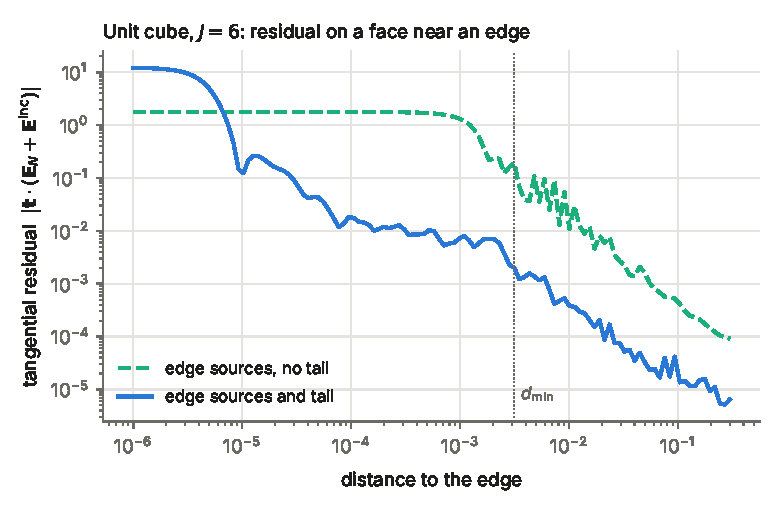
\includegraphics[width=0.6\textwidth]{fig_edge_residual.pdf}
  \caption{Unit cube, $J = 6$, one depth per octave: tangential residual on a face as a function of the distance to an edge, away from the vertices, with and without the tail. The dotted line marks the deepest free depth $d_J$.}
  \label{fig:edgeresidual}
\end{figure}

\section{Exponents at a conical point}
\label{sup:cone}

Near the vertex of a perfectly conducting cone the field is a sum of terms of two types \cite{vanbladel1996,desmedt1986,costabel2000},
\begin{equation}
  \bE = \nabla\bigl(r^{\nu}\,Y(\hat\bx)\bigr), \qquad \bH = \nabla\bigl(r^{\tau}\,Z(\hat\bx)\bigr),
\end{equation}
where $Y$ and $Z$ are eigenfunctions of the Laplace--Beltrami operator on the part of the unit sphere outside the cone, with Dirichlet and Neumann conditions and eigenvalues $\nu(\nu+1)$ and $\tau(\tau+1)$. The electric type gives $\bE\sim r^{\nu-1}$. The magnetic type gives $\bH\sim r^{\tau-1}$ and $\bE\sim r^{\tau}$. For polyhedral corners these are the principal singular parts of the time-harmonic field found by Costabel and Dauge \cite[Section 6.6]{costabel2000}.

We compute the eigenvalues by the method of particular solutions in its stable form \cite{betcke2005}. For a trial value of $\nu$ the functions $P_\nu(-\hat\bx\cdot\mathbf{s}_j)$, with $P_\nu$ the Legendre function and $\mathbf{s}_j$ a point of the sphere inside the cone, satisfy the eigenvalue equation on the sphere away from $\mathbf{s}_j$. They are the fundamental solutions of the sphere. The value $\nu$ is an exponent when a combination of them vanishes on the boundary curve without vanishing in the domain. For the almond tip the poles $\mathbf{s}_j$ lie on the focal segment of the elliptic cross-section and cluster towards its ends. For the cube corner they lie inside the spherical triangle that the cube cuts out and cluster exponentially towards its three corners. For a circular cone, where the exponent is known as a root of a Legendre function, the method reproduces it to eight digits.

\emph{Cube vertex.} For the exterior of a corner of the cube we obtain $\nu = 0.45417$, $1.23087$ and $\tau = 0.840$, $1.20635$. De Smedt and Van Bladel \cite{desmedt1986} give $\nu = 0.45410$ and $\tau = 0.84108$ for the rectangular corner (their Table V).

\emph{Almond tip.} The tip is an elliptic cone with half-angles $34.09^\circ$ and $12.71^\circ$, that is, with axis ratio $1/3$. \autoref{tab:coneexp} lists the exponents by the parities of the potential under the two mirrors of the almond. Only one exponent is below $0.87$, $\nu = 0.29959$, and it belongs to the class that is even under both mirrors. The values are unchanged in five digits when the number of poles is varied from $12$ to $36$. Bilinear interpolation in Tables I, III and IV of \cite{desmedt1986} gives $\nu = 0.298$ and $\tau = 0.885$ and $0.967$ for this cone, against our $0.29959$, $0.87905$ and $0.96803$. The differences of up to $0.7\%$ are of the size of the accuracy stated there.

\begin{table}[htbp]
  \centering
  \caption{Exponents of the elliptic cone at the tip of the almond, by the parities of the potential under the mirrors $y\to-y$ and $z\to-z$.}
  \label{tab:coneexp}
  \begin{tabular}{lll}
    \toprule
    Parity $(y,z)$ & $\nu$ (electric type) & $\tau$ (magnetic type) \\
    \midrule
    even, even & $\mathbf{0.29959}$, $1.46427$ & $1.05604$, $1.98580$ \\
    odd, even  & $1.10372$, $2.24730$ & $0.96803$, $1.96545$ \\
    even, odd  & $1.04120$, $2.10576$ & $0.87905$, $1.75454$ \\
    odd, odd   & $2.01295$, $3.04849$ & $1.97538$, $2.90094$ \\
    \bottomrule
  \end{tabular}
\end{table}

\emph{From exponents to weights.} The tail sources lie on rows that run into the conical point with spacing proportional to the distance $r$. Dipoles of strength $r^{e}$ on such a row produce a field that scales like $r^{e-3}$. A field $r^{\nu-1}$ therefore needs electric dipoles with $e = \nu+2$, and the magnetic type needs magnetic dipoles with $e = \tau+2$.

\section{The singular set of the torus}
\label{sup:torus}

We give two arguments and two numerical tests for the bound (10) of the paper, $a_s > R - \sqrt{R^2-a^2}$. None is a proof for Maxwell's equations.

\emph{Images.} A plane through the axis cuts the tube in two discs of radius $a$ whose centres are $2R$ apart. For one disc, the singularity at the centre of the other is an exterior source. Its image in the first disc lies at the distance $a^2/(2R)$ from the centre, on the side of the axis. The image of this image lies at $a^2/(2R - a^2/(2R))$, and so on. The sequence $\delta\mapsto a^2/(2R-\delta)$ increases to its fixed point $\delta = R - \sqrt{R^2-a^2}$. The singularities therefore accumulate at the focal ring.

\emph{Static limit.} For Laplace's equation the exterior field of the torus is a series of toroidal harmonics, each of which is singular only on the focal ring.

\emph{Decay of the source density.} The decay of the Fourier coefficients of the dipole density around a source circle gives the distance from the centre of the circle to the nearest singularity. For $a/R = 0.8$ the fitted distance is between $0.39$ and $0.40$ for four different incident waves and two wavenumbers, and the predicted value is $R - \sqrt{R^2-a^2} = 0.40$.

\emph{Coefficient growth.} With a fixed number of sources, the norm of the coefficients stays of order one while $a_s$ satisfies the bound and grows by orders of magnitude below it (Figure 2 of the paper). For $a/R = 0.8$ it is $3.6$ at $a_s/a = 0.5$ and $7\times10^{4}$ at $a_s/a = 0.4$.

\emph{What the literature covers.} Millar \cite{millar1983} gives the complex Riemann function of the axially symmetric Helmholtz equation and a continuation formula for bodies whose meridian curve meets the axis, with the prolate spheroid as the worked example. The torus is outside this setting. For tori in four and six dimensions, Aberra \cite{aberra2002} shows that the Schwarz potential is singular only on the circle traced by the centre of the generating disc. In three dimensions the Riemann function has a logarithmic term on the axis, which is absent in even dimensions \cite{millar1983}, and it is through the axis that the far side of the tube acts in our image argument. A proof of the bound is open.

\section{Evaluation of the line sources}
\label{sup:lines}

A line source at depth $d$ carries a polynomial density in the stretched variable $u$, and each matrix entry is the integral of a dipole field against one mode. The integrand varies on the scale of the distance between the target and the line, which ranges from $d/3$ to the size of the cube. We organise the quadrature so that most of the work is shared between the targets.

The interval $-1\le u\le1$ is divided into a binary tree of panels, and each panel carries a fixed set of nodes. On the four coarsest levels a panel is wide compared with the scale on which the modes vary. There we use $12$ Gauss nodes in the physical variable $t$ and replace the kernel by its polynomial interpolant, so that the weights are the exact moments of the Lagrange polynomials against the modes. On the finer levels we use $8$ Gauss nodes in $u$. All nodes and weights are computed once for each depth. A target descends the tree and accepts a panel as soon as the length of the panel is smaller than its distance from the target. A distant target then needs $12$ kernel values for the whole line, and a target at distance $d$ needs a few hundred. The electric and the magnetic line at the same position share the kernel values. The lines of a tail share the nodes, and their kernel values are summed with the tail weights before the modes are accumulated. The eight mirror images of a target are processed together, and their signed sums are written to the matrices of the parity classes in one pass.

With $20$ and $10$ nodes in place of $12$ and $8$ the fields of Table 1 of the paper change by less than $10^{-6}$, and by less than $10^{-7}$ up to $J = 10$. These node numbers are for a side of one wavelength. They must grow with the wavenumber, because the phase of the kernel varies along a panel in proportion to $k$. At two wavelengths we use $20$ and $10$ nodes, which changes the fields by less than $10^{-10}$ against $32$ and $14$. With $12$ and $8$ the fields there are wrong by up to $2\times10^{-4}$.

\section{Boundary element settings}
\label{sup:bempp}

We used Bempp-cl version 0.4.2 \cite{betcke2021}. The electric field integral equation is discretised with Rao--Wilton--Glisson functions as trial functions and scaled N\'ed\'elec functions as test functions. The dense matrix is assembled in double precision, and the system is solved by LU factorisation with LAPACK.

\emph{Backend.} Bempp-cl has two assembly backends. We ran the OpenCL backend on the processor through the PoCL driver. It assembled the matrices of this paper about twenty times faster than the Numba backend, with identical results. For a sphere with $4824$ unknowns the assembly took $4.3$\,s against $96$\,s.

\emph{Quadrature and meshes for the cube.} The quadrature orders of the library are $4$ for regular and $6$ for singular integrals by default, and we also used the orders $6$ and $8$, and $8$ and $10$. The graded meshes use a tensor grid on each face with the nodes $\pm\tfrac12\bigl(1-(1-|\xi|)^{g}\bigr)$, $\xi$ equally spaced in $[-1,1]$, and each rectangle is cut into two triangles. We scanned the grading exponent $g$ between $1.25$ and $2.25$ together with the three quadrature settings and seven mesh sizes. \autoref{tab:bemenv} lists the runs that no faster run beats. With the default quadrature the error is not monotone in $g$, which suggests that the quadrature error and the mesh error partly cancel at the best values. The curve for Bempp in the cost figure of the paper is this lower envelope.

\begin{table}[htbp]
  \centering
  \caption{Unit cube, $k = 2\pi$, standard wave: the fastest Bempp runs with the mirror symmetry for each accuracy, over all gradings $g$, quadrature orders and mesh sizes that we tried. Difference from the MFS reference.}
  \label{tab:bemenv}
  \small
  \begin{tabular}{rlrrl}
    \toprule
    $g$ & Quadrature & Unknowns & Time [s] & Error \\
    \midrule
\tablebody{cube_bem_env}
    \bottomrule
  \end{tabular}
\end{table}

\emph{Mirror symmetry.} Bempp does not use the symmetry of a body. To compare on an equal footing we solved the boundary element system of the cube with the three mirror planes ourselves. The graded mesh is built so that it is invariant under the eight reflections. A reflection then acts on the Rao--Wilton--Glisson coefficients as a signed permutation, and a current of a given parity class is a combination of symmetrised basis functions, one for each orbit of basis functions under the reflections. We assemble only the rows of the matrix that belong to the test functions of one octant, which Bempp allows by restricting the test space to a part of the mesh. The rows are folded with the symmetrised basis, and each class is solved by an LU factorisation of an eighth of the size. The solution differs from that of the full system by $3\times10^{-5}$ with the default quadrature and by $2\times10^{-6}$ with the orders $8$ and $10$, because the quadrature rules of the library are not invariant under the reflections. With the symmetry the boundary element solution is obtained $3.5$ to $8$ times faster, and meshes with up to $28800$ unknowns fit into memory. Without it the OpenCL driver limits a single matrix to $4$\,GB on our machine, which is $16384$ unknowns.

\section{Further results}
\label{sup:tables}

\subsection{Sphere, torus and almond}

Tables~\ref{tab:sphere} to \ref{tab:almond} list the runs behind panels (a) to (c) of the cost figure of the paper. For the torus, the MFS with the full matrix does not use the rotational symmetry.

\begin{table}[htbp]
  \centering
  \caption{Unit sphere, $k = 2\pi$: unknowns, wall time and error against the Mie series. MFS with $R = 0.5$; Bempp on quasi-uniform meshes.}
  \label{tab:sphere}
  \small
  \begin{tabular}{lrrl}
    \toprule
    Method & Unknowns & Time [s] & Error \\
    \midrule
\tablebody{sphere}
    \bottomrule
  \end{tabular}
\end{table}

\begin{table}[htbp]
  \centering
  \caption{Torus, $R = 1$, $a = 0.5$, $k = 2\pi$, wave along the axis: unknowns, wall time and difference from the finest MFS run.}
  \label{tab:torus}
  \small
  \begin{tabular}{lrrl}
    \toprule
    Method & Unknowns & Time [s] & Error \\
    \midrule
\tablebody{torus}
    \bottomrule
  \end{tabular}
\end{table}

\begin{table}[htbp]
  \centering
  \caption{NASA almond, $1.19$\,GHz, nose-on incidence: unknowns, wall time and difference from the finest MFS layout ($8{:}5$).}
  \label{tab:almond}
  \small
  \begin{tabular}{lrrl}
    \toprule
    Method & Unknowns & Time [s] & Error \\
    \midrule
\tablebody{almond}
    \bottomrule
  \end{tabular}
\end{table}

\subsection{Cube: Bempp with the grading $g = 2$}

\autoref{tab:cubebem} lists Bempp on quasi-uniform meshes and on meshes graded with $g = 2$, without and with the mirror symmetry. On quasi-uniform meshes the edge singularity limits the rate. With the default quadrature the graded meshes with $g = 2$ stall near $8\times10^{-4}$, and beyond $14112$ unknowns the convergence slows for all settings.

\begin{table}[htbp]
  \centering
  \caption{Unit cube, standard wave: Bempp on quasi-uniform meshes and on meshes graded towards the edges with $g = 2$, for three choices of the quadrature orders (regular/singular). Unknowns, difference from the MFS reference, and wall time without and with the mirror symmetry.}
  \label{tab:cubebem}
  \small
  \begin{tabular}{llrlrr}
    \toprule
    Mesh & Quadrature & Unknowns & Error & \multicolumn{2}{c}{Time [s]} \\
         &            &          &       & no symmetry & symmetry \\
    \midrule
\tablebody{cube_bem}
    \bottomrule
  \end{tabular}
\end{table}

\subsection{Cube: a general incident wave}

A wave from a general direction excites all eight parity classes. We tested the wave that arrives from the polar angle $60^\circ$ and the azimuth $25^\circ$, with its polarisation rotated by $35^\circ$ from the plane of incidence (\autoref{tab:cubeoblique}). The reference is the MFS run with two depths per octave at $J = 10$ for this wave. For the MFS the assembly is shared between the classes and eight factorisations are needed instead of two. For the boundary element method with symmetry the cost hardly changes.

\begin{table}[htbp]
  \centering
  \caption{Unit cube, oblique wave: MFS with eight parity classes, and Bempp on meshes graded with $g = 2$ without and with the mirror symmetry. Unknowns (for the MFS, all classes together), wall time and difference from the MFS reference.}
  \label{tab:cubeoblique}
  \small
  \begin{tabular}{lrrl}
    \toprule
    Method & Unknowns & Time [s] & Error \\
    \midrule
\tablebody{cube_oblique}
    \bottomrule
  \end{tabular}
\end{table}

\subsection{Cube: two and three wavelengths}

At $k = 4\pi$ the layout is the same as at $k = 2\pi$ except that the interior panels of the boundary grid are half as long, each line carries four more modes, and the line quadrature uses more nodes (\autoref{sup:lines}). \autoref{tab:cubek} lists the results for the standard wave. For the oblique wave of \autoref{tab:cubeoblique} the MFS with one depth per octave needs $12$, $18$ and $28$\,s for errors of $1.5\times10^{-3}$, $6.4\times10^{-4}$ and $2.7\times10^{-4}$.

At $k = 6\pi$ the base grid and its depth must follow the wavelength as well: the first depth is $0.2/3$ and the base grid has $18$ points per face. With one depth per octave the errors at $J = 6$, $7$ and $8$ are $2.0\times10^{-3}$, $1.3\times10^{-3}$ and $8.6\times10^{-4}$ after $21$, $25$ and $32$\,s, measured against the run with two depths per octave at $J = 8$. Bempp with symmetry, graded with $g = 1.5$, needs $23$\,s for $1.0\times10^{-3}$ and $56$\,s for $6.9\times10^{-4}$. We have not tuned this case.

\begin{table}[htbp]
  \centering
  \caption{Unit cube at $k = 4\pi$ (side of two wavelengths), standard wave: MFS with one and two source depths per octave, and Bempp on meshes graded with $g = 2$ with the mirror symmetry. Unknowns (for the MFS, per parity class; two classes are solved), wall time and difference from the MFS run with two depths per octave at $J = 10$.}
  \label{tab:cubek}
  \small
  \begin{tabular}{lrrl}
    \toprule
    Method & Unknowns & Time [s] & Error \\
    \midrule
\tablebody{cube_k2}
    \bottomrule
  \end{tabular}
\end{table}

\bibliographystyle{elsarticle-num}
\bibliography{refs}

\end{document}
